\chapter{METODOLOGI PENENILITIAN}
\section{Metode Penelitian}
\subsection{Metode Pengumpulan Data}

Dalam penelitian ini, metode pengumpulan data yang digunakan meliputi studi pustaka, wawancara, dan observasi. Ketiga metode ini akan memberikan kontribusi yang beragam dalam mendapatkan informasi yang diperlukan untuk penelitian.

\begin{enumerate}[leftmargin=1cm, itemindent=0.6cm,labelwidth=15pt, labelsep=5pt, listparindent=1cm,align=left]

    \item Studi Pustaka

    Studi pustaka merupakan metode yang penting dalam proses penelitian ini. Melalui studi pustaka, peneliti akan mengumpulkan informasi dari sumber-sumber yang relevan, seperti buku dan jurnal ilmiah. Dalam konteks pengembangan media pembelajaran pengolahan citra digital menggunakan visualisasi interaktif berbasis web, studi pustaka akan memberikan pemahaman yang mendalam tentang konsep pengolahan citra digital, prinsip-prinsip desain pembelajaran, dan teknologi terkait pengembangan aplikasi web.

    \item Wawancara

    Metode wawancara akan digunakan untuk mendapatkan perspektif dan informasi dari para ahli dalam bidang pengolahan citra digital. Wawancara akan dilakukan dengan para akademisi atau praktisi yang memiliki pengetahuan dan pengalaman dalam pengolahan citra digital. Pertanyaan-pertanyaan terkait dengan konsep pengolahan citra digital, penggunaan visualisasi interaktif dalam pembelajaran, tantangan yang dihadapi dalam pengembangan media pembelajaran, dan saran atau rekomendasi akan diajukan kepada responden.

    \item Observasi

    Metode observasi dilakukan dengan mengamati penggunaan media pembelajaran yang ada atau situasi pembelajaran yang terkait dengan pengolahan citra digital. Observasi dilakukan secara langsung untuk melihat bagaimana mahasiswa berinteraksi dengan materi pembelajaran, sejauh mana mereka memahami konsep-konsep pengolahan citra digital, serta kendala atau masalah yang mungkin timbul selama proses pembelajaran. Observasi ini dilakukan dalam lingkungan kelas atau laboratorium komputer.

\end{enumerate}

\subsection{Metode Pengembangan Aplikasi}
Metode pengembangan aplikasi yang akan digunakan dalam penelitian ini adalah metode waterfall. Metode waterfall adalah salah satu pendekatan pengembangan perangkat lunak yang terstruktur dan linear, di mana setiap fase pengembangan dilakukan secara berurutan dan tidak ada overlap antar fase. Berikut adalah tahapan-tahapan pengembangan aplikasi menggunakan metode waterfall:

\subsubsection{Analisis Kebutuhan}

    Tahap analisis kebutuhan dilakukan untuk memahami secara mendalam kebutuhan pengguna dan tujuan dari pengembangan aplikasi. Pada tahap ini, dilakukan identifikasi kebutuhan pengolahan citra digital yang perlu disajikan dalam media pembelajaran berbasis web. Analisis kebutuhan ini melibatkan wawancara dengan para pengguna potensial dan pengumpulan informasi terkait konsep-konsep pengolahan citra digital yang penting.

\subsubsection{Perancangan}

    Setelah kebutuhan dianalisis, tahap perancangan dilakukan untuk merancang struktur dan fungsionalitas media pembelajaran. Pada tahap ini, dilakukan perancangan antarmuka pengguna, aliran informasi, dan navigasi aplikasi. Perancangan ini juga melibatkan pemilihan algoritma pengolahan citra yang akan digunakan dalam media pembelajaran.

\begin{enumerate}[leftmargin=1cm, itemindent=0.6cm,labelwidth=15pt, labelsep=5pt, listparindent=1cm,align=left]

\item\textit{Context Diagram}

\textit{Context diagram} adalah sebuah diagram yang digunakan untuk menggambarkan sistem secara keseluruhan serta hubungannya dengan entitas eksternal yang berinteraksi dengan sistem tersebut. Diagram ini memberikan pandangan menyeluruh mengenai sistem tanpa menyelidiki detail internalnya. Pada context diagram, sistem digambarkan dengan sebuah lingkaran atau persegi panjang di tengah diagram, sementara entitas eksternal digambarkan dengan bentuk yang berbeda di sekitarnya. Hubungan antara sistem dan entitas eksternal ditunjukkan dengan garis yang menghubungkan mereka, menggambarkan aliran data atau informasi.

          \begin{figure*}[ht]
    	      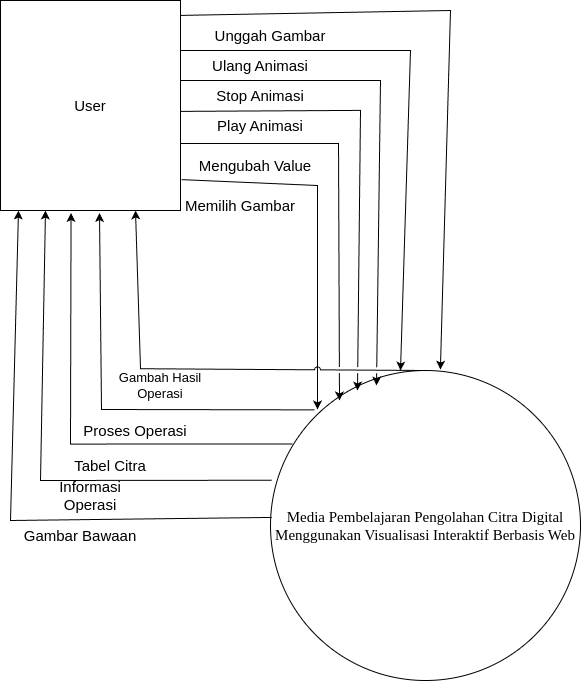
\includegraphics[width=0.6\textwidth, center]{images/diagram-konteks2.png}
              \caption{\textit{Context Diagram} Media Pembelajaran pengolahan Citra Menggunakan Visualisasi Interaktif Berbasis Web}
          \end{figure*}

\textit{Context diagram} sangat berguna pada tahap awal perancangan sistem karena membantu para pemangku kepentingan memahami batasan dan lingkup sistem. Diagram ini juga memudahkan identifikasi entitas eksternal yang berinteraksi dengan sistem, seperti pengguna, perangkat lunak lain, atau sistem fisik. Dengan demikian, context diagram membantu menentukan kebutuhan fungsional dan non-fungsional sistem, serta menyekjdiakan dasar untuk perancangan lebih detail. Adapun Context diagram pada aplikasi media pembelajaran pengolahan citra digital berbasis web bisa dilihat pada gambar 3.1.


\item\textit{Hierarchy Chart}

\textit{Hierarchy chart} adalah sebuah alat visual yang digunakan untuk menggambarkan struktur hirarkis suatu sistem atau proses, menampilkan hubungan antara komponen atau modul dalam bentuk hierarki. Diagram ini sering digunakan dalam pengembangan perangkat lunak, perencanaan organisasi, dan manajemen proyek untuk memberikan pemahaman yang jelas mengenai bagaimana berbagai elemen berinteraksi dan berhubungan satu sama lain. \textit{Hierarchy chart} yang akan dibangun bisa dilihat pada gambar 3.2.

          \begin{figure*}[ht]
    	      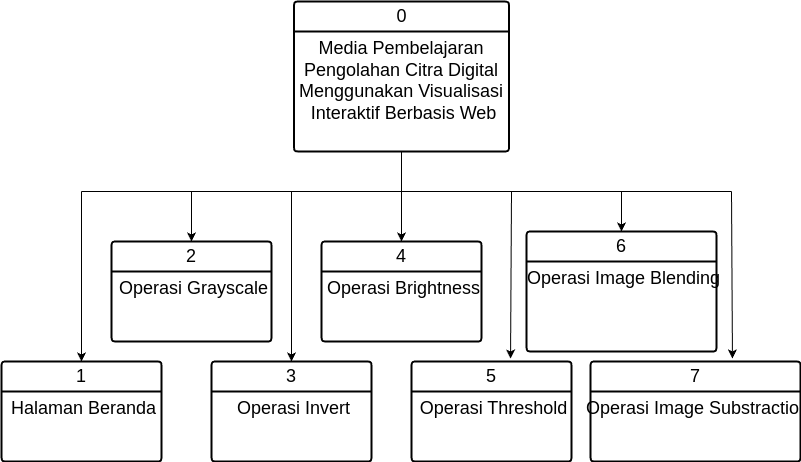
\includegraphics[width=15cm, center]{images/Hierarchy-Chart.png}
              \caption{\textit{Hierarchy Chart} Media Pembelajaran pengolahan Citra Menggunakan Visualisasi Interaktif Berbasis Web}
          \end{figure*}

\item\textit{Activity Diagram}

\textit{Activity diagram} adalah salah satu jenis diagram dalam Unified Modeling Language (UML) yang sangat berguna dalam memodelkan alur kerja atau proses bisnis yang terjadi di dalam sebuah sistem. Diagram ini memberikan representasi visual yang jelas dari berbagai aktivitas serta urutan tindakan yang berlangsung dalam sebuah proses, memperlihatkan bagaimana satu aktivitas mengarah dan bertransisi ke aktivitas lainnya. Hal ini, seperti yang dapat dilihat pada gambar 3.3, membantu dalam memahami serta menganalisis alur kerja secara lebih mendalam dan terstruktur.

       
          \begin{figure*}[ht]
    	      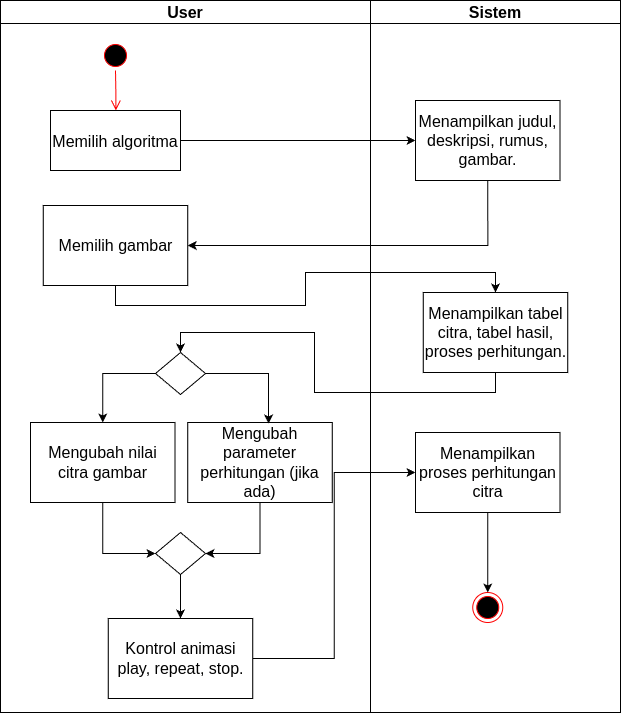
\includegraphics[width=8cm, center]{images/Activity-Diagram2.png}
              \caption{\textit{Activity Diagram} Media Pembelajaran pengolahan Citra Menggunakan Visualisasi Interaktif Berbasis Web}
          \end{figure*}

      \item Program \textit{Flowchart}

Berikut adalah flowchart yang menunjukkan sistem media pembelajaran pengolahan citra digital berbasis web yang memperlihatkan alur atau langkah-langkah yang terjadi dalam sistem tersebut. Flowchart tersebut merupakan gambaran visual tentang bagaimana sistem media pembelaran tersebut beroperasi.

\begin{enumerate}[leftmargin=1cm, itemindent=0.6cm,labelwidth=15pt, labelsep=5pt, listparindent=1cm,align=left]

    \item Program Flowchart Operasi Grayscale

        Flowchart Operasi Grayscale adalah sebuah gambaran langkah demi langkah saat pengguna melakukan memulai proses mengubah tabel citra warna menjadi citra grayscale. Pada menu grayscale pengguna diminta memilih salah satu dari gambar kemudian pengguna bisa mengubah nilai dari citra warna tersebut. Jika pengguna tidak mengubah nilai dari citra warna pengguna bisa menekan tombol \textit{start, pause, stop} dan \textit{repeat}.

          \begin{figure*}[ht]
    	      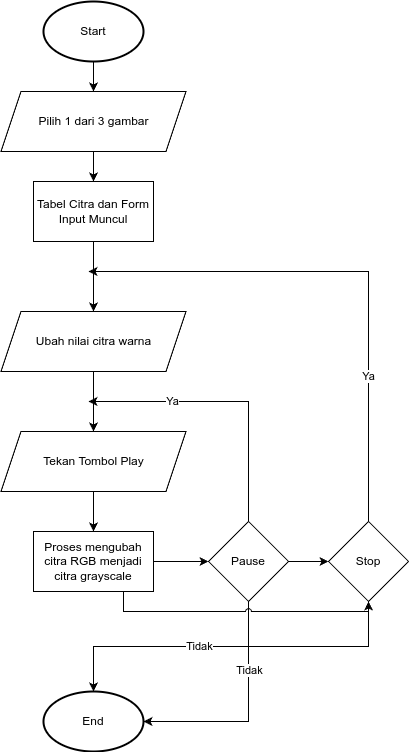
\includegraphics[width=0.5\textwidth, center]{images/flowchart-grayscale.png}
              \caption{\textit{Flowchart grayscale}}
          \end{figure*}

    \item Program Flowchart Operasi \textit{Invert}

        Flowchart Operasi \textit{Invert} atau negatif adalah sebuah gambaran langkah demi langkah saat pengguna melakukan memulai proses mengubah tabel citra grayscale menjadi citra negatif. Pada menu \textit{invert} pengguna diminta memilih salah satu dari gambar kemudian pengguna bisa mengubah nilai dari citra warna tersebut. Jika pengguna tidak mengubah nilai dari citra warna pengguna bisa menekan tombol \textit{start, pause, stop} dan \textit{repeat}.


      \begin{figure*}[ht]
          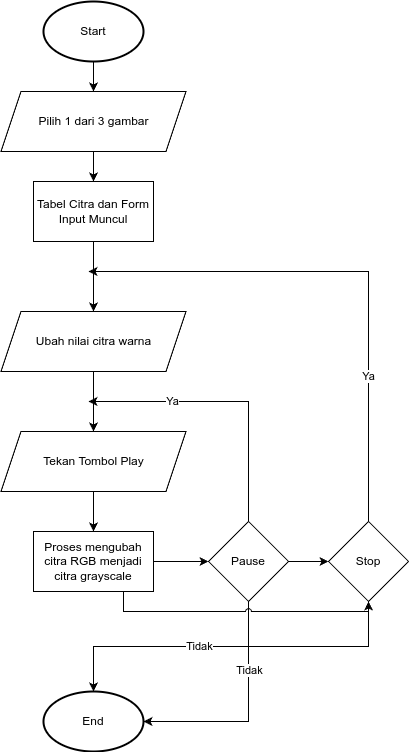
\includegraphics[width=0.5\textwidth, center]{images/flowchart-grayscale.png}
          \caption{\textit{Flowchart Invert}}
      \end{figure*}

    \pagebreak

    \item Program Flowchart Operasi \textit{Brightness}

    Flowchart Operasi \textit{Brightness} adalah sebuah gambaran langkah demi langkah saat pengguna melakukan memulai proses mengubah tabel citra grayscale menjadi citra dengan nilai baru yaitu peningkatan kecerahan. Pada menu \textit{brightness} pengguna diminta memilih salah satu dari gambar kemudian pengguna bisa mengubah nilai dari citra grayscale tersebut. Jika pengguna tidak mengubah nilai dari citra warna pengguna bisa menekan tombol \textit{start, pause, stop} dan \textit{repeat}. Pengguna juga bisa mengatur berapa besar konstanta yang akan ditingkatkan menggunakan \textit{slider ranger input}.

    \pagebreak

      \begin{figure*}[ht]
          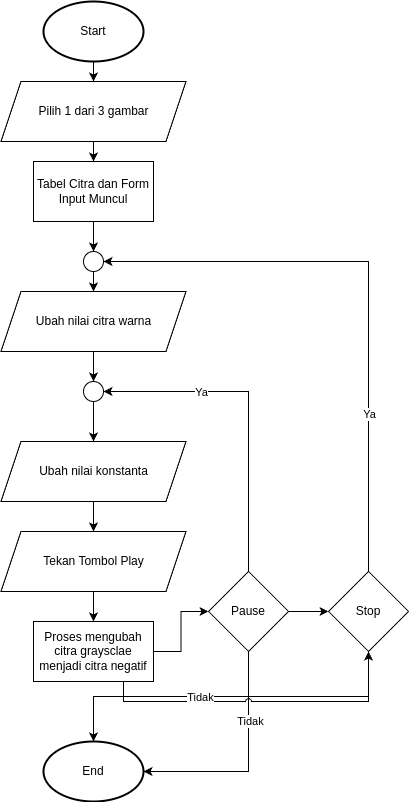
\includegraphics[width=0.5\textwidth, center]{images/flowchart-brightness.png}
          \caption{\textit{Flowchart Brightness}}
      \end{figure*}

    \item Program Flowchart Operasi \textit{Threshold}

    Flowchart operasi \textit{threshold} adalah sebuah gambaran langkah demi langkah saat pengguna melakukan memulai proses mengubah tabel citra grayscale menjadi citra dengan antara 0 atau 255. Pada menu \textit{threshold} pengguna diminta memilih salah satu dari gambar kemudian pengguna bisa mengubah nilai dari citra grayscale tersebut. Jika pengguna tidak mengubah nilai dari citra warna pengguna bisa menekan tombol \textit{start, pause, stop} dan \textit{repeat}. Pengguna juga bisa mengatur berapa besar nilai \(T\) yang akan ditingkatkan menggunakan \textit{input number}.

    \pagebreak

      \begin{figure*}[ht]
          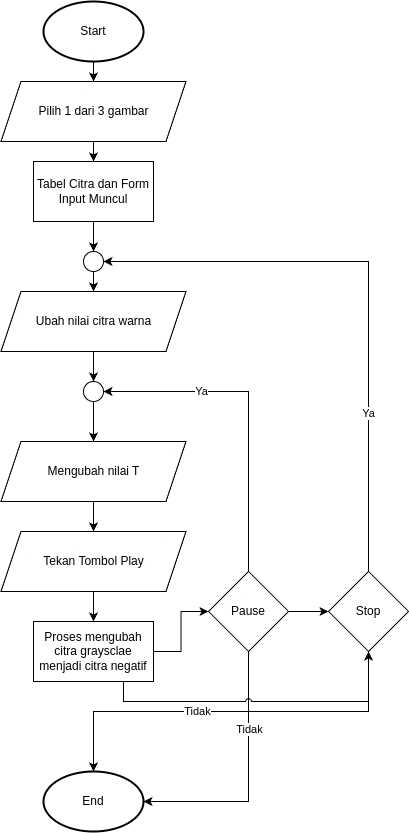
\includegraphics[width=0.5\textwidth, center]{images/flowchart-threshold.png}
          \caption{\textit{Flowchart Threshold}}
      \end{figure*}

    \item Program Flowchart Operasi \textit{Image Blending}

        Flowchart Operasi \textit{Image Blending} adalah sebuah gambaran langkah demi langkah saat pengguna melakukan memulai proses penjumlahan antara 2 citra grayscale. Pada menu \textit{image blending} pengguna diminta memilih 2 gambar kemudian pengguna bisa mengubah nilai dari citra grayscale tersebut. Jika pengguna tidak mengubah nilai dari citra warna pengguna bisa menekan tombol \textit{start, pause, stop} dan \textit{repeat}. Pengguna juga bisa mengatur berapa besar nilai \(\alpha\) antara 0.1 sampai dengan 0.9 menggunakan \textit{input number}
    \pagebreak

      \begin{figure*}[ht]
          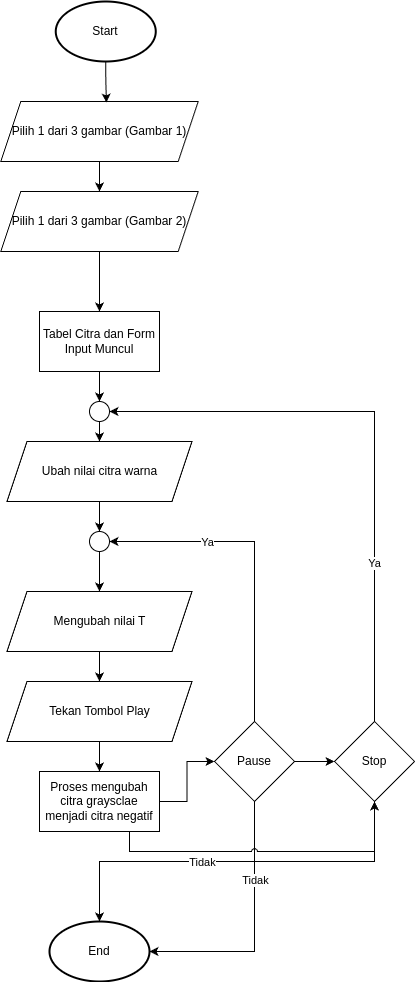
\includegraphics[width=0.5\textwidth, center]{images/flowchart-blending.png}
          \caption{\textit{Flowchart Image Blending}}
      \end{figure*}

    \item Program Flowchart Operasi \textit{Image Substraction}

    Flowchart Operasi \textit{Image Substraction} atau pengurangan citra adalah sebuah gambaran langkah demi langkah saat pengguna melakukan memulai proses pengurangan antara 2 citra grayscale. Pada menu \textit{image blending} pengguna diminta memilih 2 gambar kemudian pengguna bisa mengubah nilai dari citra grayscale tersebut. Jika pengguna tidak mengubah nilai dari citra warna pengguna bisa menekan tombol \textit{start, pause, stop} dan \textit{repeat}.

      \begin{figure*}[ht]
          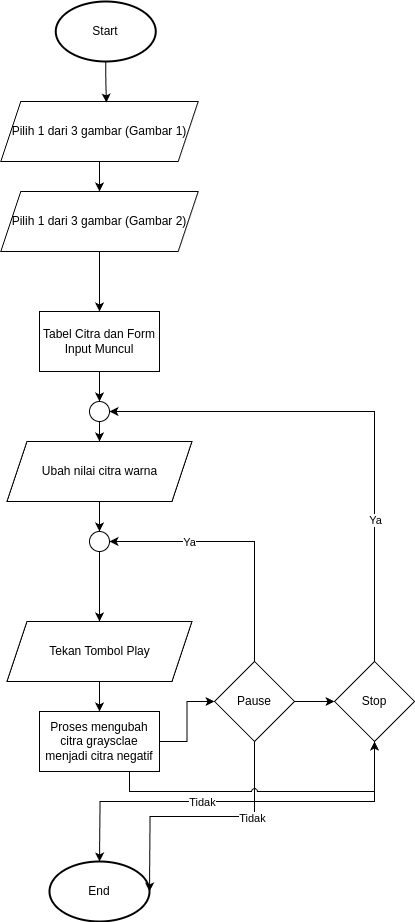
\includegraphics[width=0.5\textwidth, center]{images/flowchart-substraction.png}
          \caption{\textit{Flowchart Image Substraction}}
      \end{figure*}
\end{enumerate}

\item Desain Input

Desain input mengacu pada pengembangan antarmuka sistem yang melibatkan form input untuk pemrosesan operasi dan informasi yang inputkan akan mempengaruhi pada proses operasi itu sendiri.


\begin{enumerate}[leftmargin=1cm, itemindent=0.6cm,labelwidth=15pt, labelsep=5pt, listparindent=1cm,align=left]

    \item Desain input operasi \textit{grayscale}

Halaman ini adalah visualisasi pengolahan citra digital yang bertujuan mengubah gambar berwarna RGB menjadi grayscale. Terdapat beberapa elemen utama di halaman ini, mulai dari judul "Operasi RGB ke Grayscale" hingga deskripsi singkat tentang konversi warna.

Pengguna dapat memilih salah satu dari tiga gambar untuk diproses. Setelah memilih gambar, tabel RGB muncul dengan nilai awal, dan pengguna dapat mengubah nilai RGB melalui input text area.

          \begin{figure*}[ht]
    	      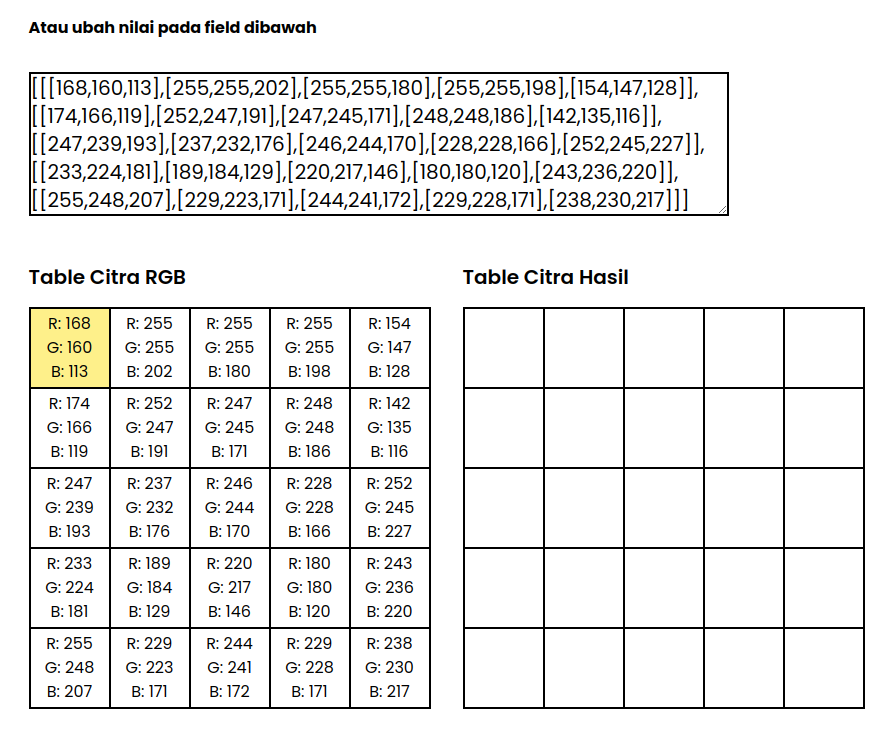
\includegraphics[width=0.6\textwidth, center]{images/input-grayscale.png}
              \caption{Desain Input Halaman \textit{Grayscale}}
          \end{figure*}

    \item Desain input operasi \textit{invert}

          \begin{figure*}[ht]
    	      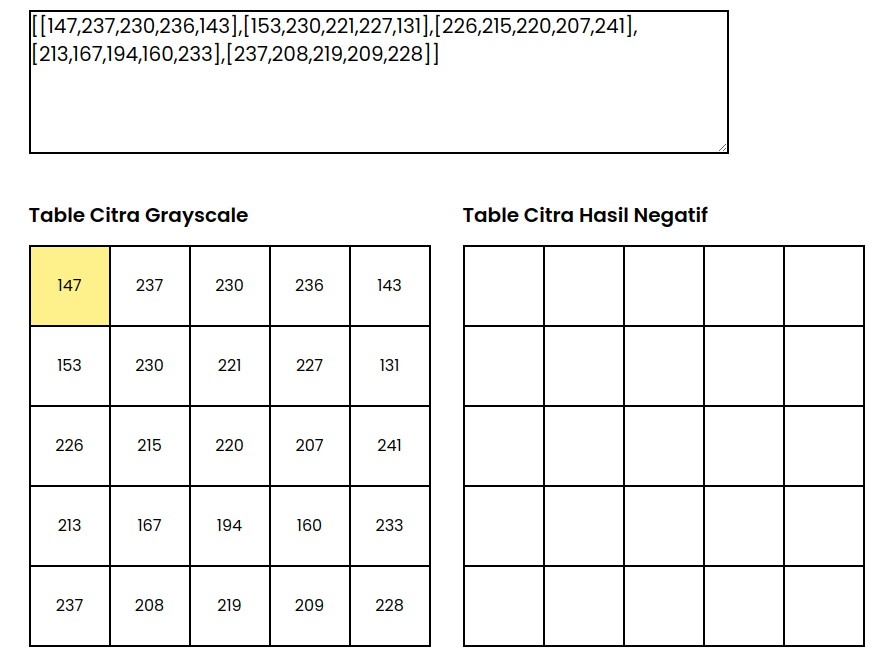
\includegraphics[width=0.6\textwidth, center]{images/input-invert.png}
              \caption{Desain Input Halaman \textit{Invert}}
          \end{figure*}

        Halaman ini adalah visualisasi pengolahan citra digital yang bertujuan mengubah gambar grayscale menjadi negatif. Terdapat beberapa elemen utama di halaman ini, mulai dari judul "Operasi Negatif", deskripsi singkat tentang konversi negatif, contoh kasus, tabel citra \textit{grayscale} serta tabel citra hasil.

Pengguna dapat memilih salah satu dari tiga gambar \textit{grayscale} untuk diproses. Setelah memilih gambar, tabel \textit{grayscale} muncul dengan nilai awal, dan pengguna dapat mengubah nilai \textit{grayscale} melalui input text area.

    \item Desain input operasi \textit{Brightness}

Untuk halaman ini yang bertujuan untuk mengubah kecerahan dari sebuah gambar. Terdapat beberapa element mulai dari judul, deskripsi singkat, rumus, tabel citra awal table citra hasil.

Pengguna dapat memilih salah satu dari tiga gambar \textit{grayscale} untuk diproses. Setelah memilih gambar, tabel \textit{grayscale} muncul dengan nilai awal, dan pengguna dapat mengubah nilai \textit{grayscale} melalui input text area. Pengguna juga dapat mengubah nilai konstanta menggunakan \textit{range slider}.

          \begin{figure*}[ht]
    	      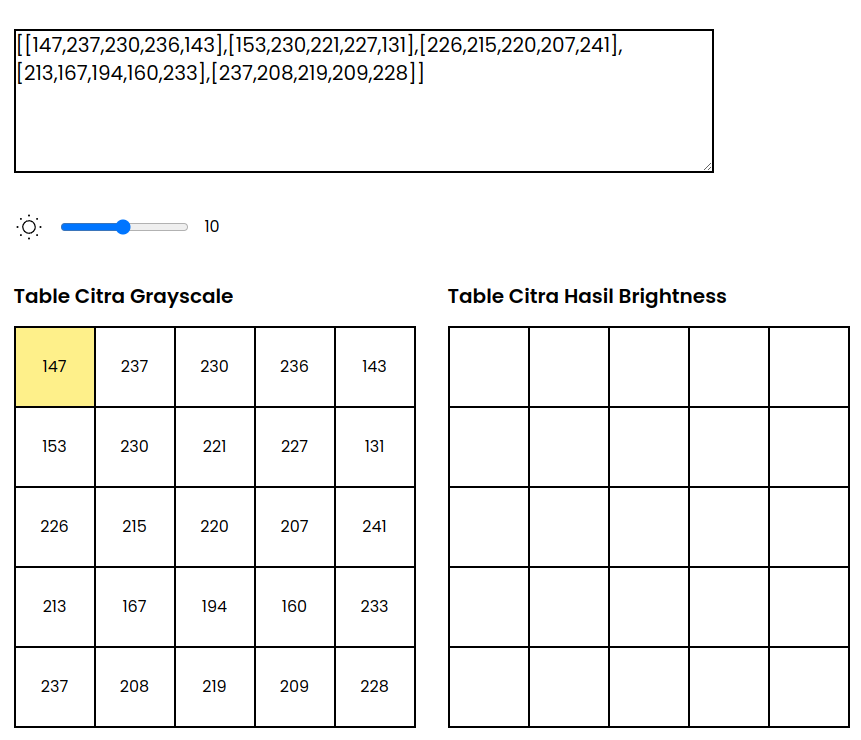
\includegraphics[width=0.6\textwidth, center]{images/input-brightness.png}
              \caption{Desain Input Halaman \textit{Brightness}}
          \end{figure*}

    \item Desain input operasi \textit{Threshold}

Pada halaman ini yang bertujuan untuk malukan proses ambang batas dari sebuah gambar. Terdapat beberapa element mulai dari judul, deskripsi singkat, rumus, tabel citra awal table citra hasil.

Pengguna dapat memilih salah satu dari tiga gambar \textit{grayscale} untuk diproses. Setelah memilih gambar, tabel \textit{grayscale} muncul dengan nilai awal, dan pengguna dapat mengubah nilai \textit{grayscale} melalui input text area. Pengguna juga dapat mengubah nilai \(T\) menggunakan \textit{input number}.

          \begin{figure*}[ht]
    	      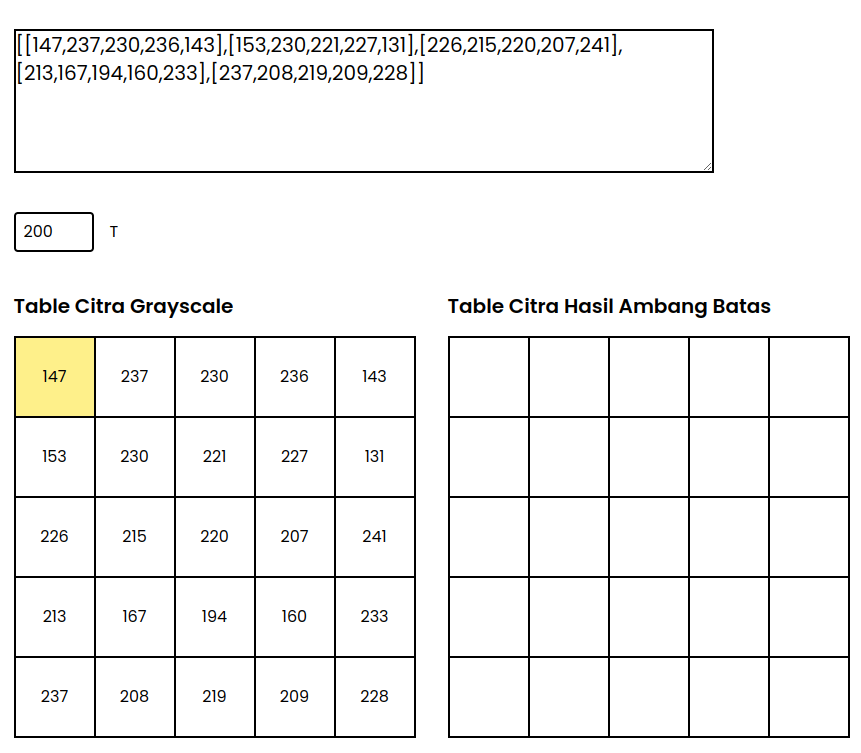
\includegraphics[width=0.8\textwidth, center]{images/input-threshold.png}
              \caption{Desain Input Halaman \textit{Threshold}}
          \end{figure*}

    \item Desain input operasi \textit{Image Blending}


          Halaman ini adalah visualisasi pengolahan citra digital yang bertujuan menggabungkan 2 buah citra. Terdapat beberapa elemen utama di halaman ini, mulai dari judul "Operasi Penjumlahan Citra", deskripsi singkat tentang \textit{image blending}, contoh kasus, 2 tabel citra \textit{grayscale} serta tabel citra hasil.

          Pengguna dapat memilih dua gambar \textit{grayscale} untuk diproses. Setelah memilih gambar, tabel \textit{grayscale} muncul dengan nilai awal, dan pengguna dapat mengubah nilai \textit{grayscale} melalui dua \textit{input text area}. Pengguna juga dapat menginput nilai \textit{threshold} dari angka 1 - 255.

\pagebreak

          \begin{figure*}[ht]
    	      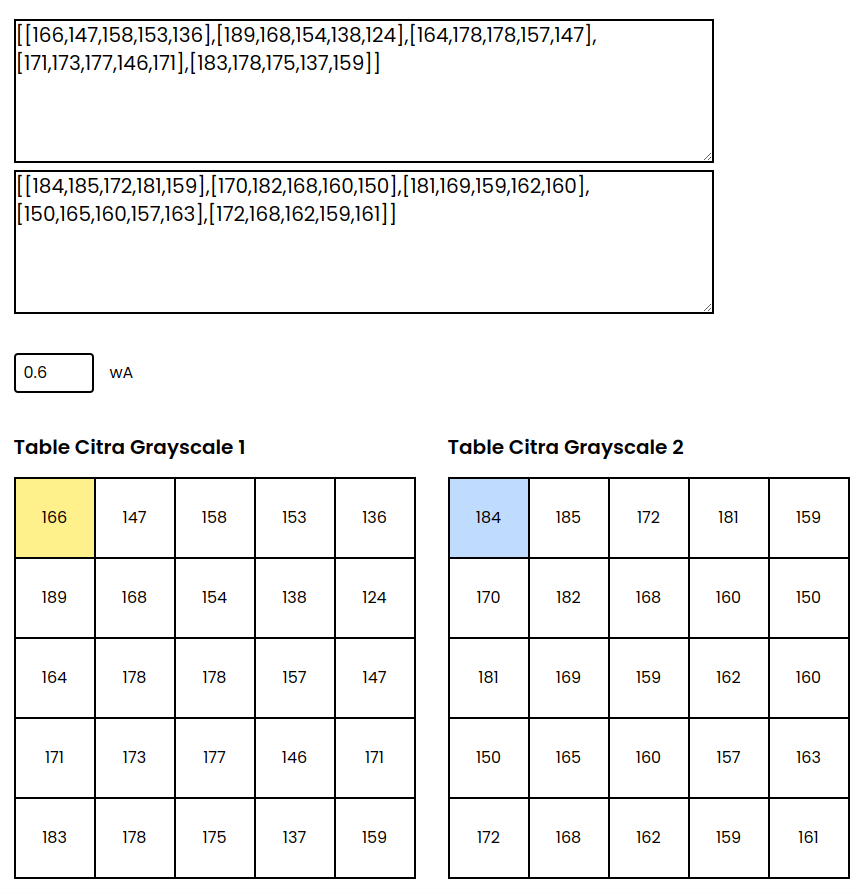
\includegraphics[width=0.6\textwidth, center]{images/input-blending.png}
              \caption{Desain Input Halaman \textit{Image Blending}}
          \end{figure*}

    \item Desain input operasi \textit{Image Substraction}

          Halaman ini adalah visualisasi pengolahan citra digital yang bertujuan mengurangi dua buah citra. Terdapat beberapa elemen utama di halaman ini, mulai dari judul "Operasi Pengurangan Citra", deskripsi singkat tentang \textit{image substraction}, contoh kasus, dua tabel citra \textit{grayscale} serta tabel citra hasil.

          Pengguna dapat memilih dua gambar \textit{grayscale} untuk diproses. Setelah memilih gambar, tabel \textit{grayscale} muncul dengan nilai awal, dan pengguna dapat mengubah nilai \textit{grayscale} melalui dua \textit{input text area}.

        \begin{figure*}[ht]
    	      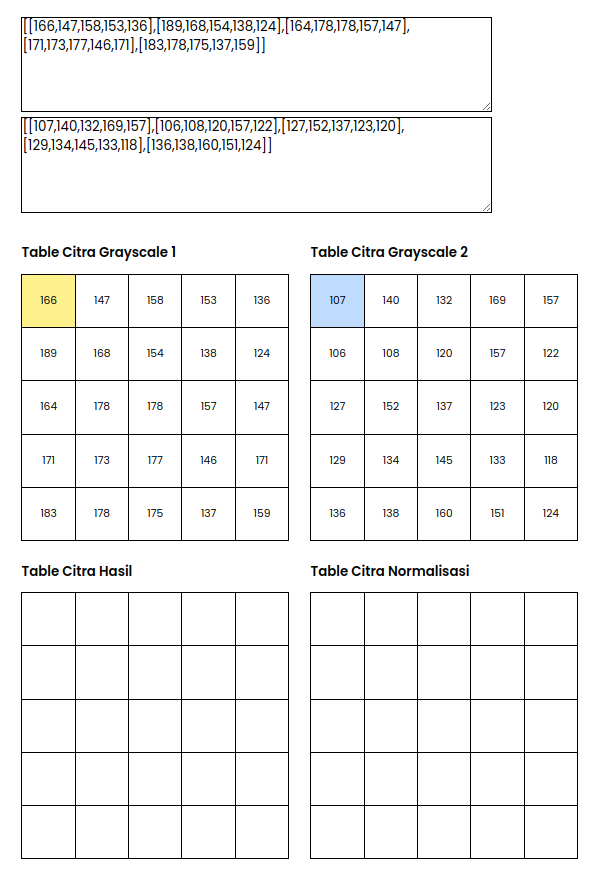
\includegraphics[width=0.6\textwidth, center]{images/input-substraction.png}
              \caption{Desain Input Halaman \textit{Image Substraction}}
        \end{figure*}

    \pagebreak

\end{enumerate}
\end{enumerate}

\subsubsection{Implementasi}

    Tahap implementasi melibatkan pembuatan kode program berdasarkan perancangan yang telah disusun sebelumnya. Pada tahap ini, dilakukan pengembangan aplikasi berbasis web yang mendukung pengolahan citra digital dan visualisasi interaktif. Web yang dibuat menggunakan HTML, CSS, dan JavaScript, dengan React dan Tailwind CSS sebagai library tambahannya. Algoritma pengolahan citra yang dipilih akan diimplementasikan dalam kode program yang sesuai.

\subsubsection{Pengujian}

        Setelah tahap implementasi, pengujian aplikasi dilakukan untuk memastikan bahwa aplikasi berfungsi dengan baik dan memenuhi kebutuhan pengguna. Pengujian ini melibatkan 30 responden yang terdiri dari mahasiswa dan masyarakat umum, yang diminta menjawab 5 pertanyaan terkait pengalaman pengguna (\textit{user experience}) dalam menggunakan aplikasi tersebut. Hasil kuisioner akan dianalisis menggunakan metode skala \textit{Likert}.

\subsubsection{Pemeliharaan}

    Setelah aplikasi diimplementasikan dan diuji, langkah selanjutnya adalah pemeliharaan. Tahap pemeliharaan melibatkan pemantauan kinerja aplikasi secara berkala dan memperbaiki masalah yang muncul setelah aplikasi berada dalam lingkungan produksi. Pemeliharaan juga mencakup penambahan fitur baru atau perubahan fungsionalitas sesuai dengan kebutuhan yang berkembang dari pengguna.

Metode waterfall memberikan pendekatan yang terstruktur dan terurut dalam pengembangan aplikasi. Setiap tahap harus diselesaikan dengan baik sebelum melanjutkan ke tahap berikutnya. Pendekatan ini memastikan bahwa setiap fase pengembangan dapat diselesaikan dengan baik sebelum melanjutkan ke fase berikutnya, sehingga mengurangi risiko perubahan yang tidak terduga.

\section{Alat dan Bahan Penelitian}
\subsection{Spesifikasi Perangkat Keras(\textit{Hardware})}
    Perangkat keras (hardware) yang digunakan dalam pembangunan aplikasi media pebelajaran yang dibuat adalah sebagai berikut:
\begin{enumerate}
    \item \textit{Procesor AMD Ryzen 7 47000U with Raden Graphics 2.00 GHz}
    \item SSD 512 GB
    \item RAM 8 GB
\end{enumerate}

\subsection{Spesifikasi Perangkat Lunak(\textit{Software})}
    Perangkat Lunak (\textit{software}) yang digunakan dalam pembangunan aplikasi lowongan kerja yang dibangun adalah sebagai berikut:

\begin{enumerate}
    \item Sistem Operasi : Arch Linux
    \item Bahasa Pemrograman : Javascript
    \item Framework : Bootstrap
    \item Aplikasi desain logika program : draw.io
    \item Code Editor : Visual Studio Code
\end{enumerate}
